\documentclass[12pt,a4paper]{article}
\usepackage[UTF8]{ctex}
\usepackage{graphicx}
\usepackage{geometry}
\usepackage{amsmath}
\usepackage{amsfonts}
\usepackage{amssymb}
\usepackage{listings}
\usepackage{xcolor}
\usepackage{float}
\usepackage{tikz}
\usepackage{fancyhdr}
\usepackage{setspace}
\usepackage{multirow}
\usepackage[most]{tcolorbox}
\tcbset{colback=white,colframe=black,boxrule=0.6pt,arc=0mm,left=3mm,right=3mm,top=2mm,bottom=2mm,breakable,enhanced}

% 下划线填空宏
\newcommand{\fillin}[1]{\underline{\makebox[8cm][l]{#1}}}
\usetikzlibrary{shapes,arrows,positioning}

\geometry{left=2.5cm,right=2.5cm,top=3.5cm,bottom=2.5cm}
\setlength{\headheight}{24.64995pt}

% 设置页眉
\pagestyle{fancy}
\fancyhf{}
\fancyhead[C]{\textbf{作业2 直线绘制算法}}
\fancyhead[R]{\thepage}
\renewcommand{\headrulewidth}{2pt}
\renewcommand{\headrule}{\hbox to\headwidth{\leaders\hrule height 2pt\hfill}}

% 设置代码样式
\lstset{
    language=C++,
    basicstyle=\ttfamily\small,
    keywordstyle=\color{blue},
    commentstyle=\color{green!50!black},
    stringstyle=\color{red},
    numbers=left,
    numberstyle=\tiny\color{gray},
    stepnumber=1,
    numbersep=5pt,
    backgroundcolor=\color{gray!10},
    showspaces=false,
    showstringspaces=false,
    showtabs=false,
    frame=single,
    tabsize=2,
    captionpos=b,
    breaklines=true,
    breakatwhitespace=false,
}

% 定义Rust语言支持
\lstdefinelanguage{Rust}{
    keywords={abstract, alignof, as, become, box, break, const, continue, crate, do, else, enum, extern, false, final, fn, for, if, impl, in, let, loop, macro, match, mod, move, mut, offsetof, override, priv, proc, pub, pure, ref, return, Self, self, sizeof, static, struct, super, trait, true, type, typeof, unsafe, unsized, use, virtual, where, while, yield},
    keywords=[2]{i8, i16, i32, i64, i128, isize, u8, u16, u32, u64, u128, usize, f32, f64, bool, char, str, String, Vec, Option, Result, Box, Rc, Arc},
    keywords=[3]{Some, None, Ok, Err, println, print, panic, assert, assert_eq, unwrap, expect},
    sensitive=true,
    morecomment=[l]{//},
    morecomment=[s]{/*}{*/},
    morestring=[b]",
    morestring=[b]',
}

\lstset{
    language=Rust,
    basicstyle=\ttfamily\small,
    keywordstyle=\color{blue}\bfseries,
    keywordstyle=[2]\color{purple},
    keywordstyle=[3]\color{teal},
    commentstyle=\color{green!50!black}\itshape,
    stringstyle=\color{red},
    numbers=left,
    numberstyle=\tiny\color{gray},
    stepnumber=1,
    numbersep=5pt,
    backgroundcolor=\color{gray!10},
    showspaces=false,
    showstringspaces=false,
    showtabs=false,
    frame=single,
    tabsize=4,
    captionpos=b,
    breaklines=true,
    breakatwhitespace=false,
    escapeinside={(*@}{@*)},
}

\title{\textbf{作业2 直线绘制算法}}
\author{程泽凯 \quad 2023112621}
\date{\today}

\begin{document}

% 自定义封面
\begin{titlepage}
    \thispagestyle{empty}
    \begin{spacing}{1.2}
    \centering
    \vspace*{10mm}
    {\zihao{4} 《计算机图形学及人机交互》\par}
    \vspace{20mm}
    {\bfseries\zihao{1} 作 业 报 告\par}
    \vspace{40mm}

    % 基本信息
    \songti\zihao{-3}
    \begin{flushleft}
    \setlength{\tabcolsep}{1em}
    \renewcommand\arraystretch{2}
    \begin{tabular}{@{}ll}
        学\quad 号： & \fillin{2023112621} \\
        姓\quad 名： & \fillin{程泽凯} \\
        年\quad 级： & \fillin{2023 级} \\
        专\quad 业： & \fillin{计算机科学与技术} \\
        院\quad 系： & \fillin{计算机与人工智能学院} \\
    \end{tabular}
    \end{flushleft}

    \vfill
    {\zihao{-3} 2025~2026 第 1 学期\par}
    \end{spacing}
\end{titlepage}

% 第二页：目录
\clearpage
\tableofcontents
\clearpage

% 正文设置
\songti\zihao{-4}
\onehalfspacing

\section{算法文字描述}

\subsection{中点画线法}

\begin{tcolorbox}

\subsubsection*{算法原理}

对于直线方程 $F(x,y) = ax + by + c = 0$，其中 $a = y_0 - y_1$，$b = x_1 - x_0$，$c = x_0y_1 - x_1y_0$。

\begin{itemize}
    \item 当 $F(x,y) = 0$ 时，点 $(x,y)$ 在直线上
    \item 当 $F(x,y) > 0$ 时，点 $(x,y)$ 在直线下方
    \item 当 $F(x,y) < 0$ 时，点 $(x,y)$ 在直线上方
\end{itemize}

\subsubsection*{决策过程}

假设当前像素为 $(x_p, y_p)$，已经确定要绘制，那么下一个像素的x坐标必然是 $x_p+1$，但y坐标有两个候选：
\begin{itemize}
    \item \textbf{右侧像素}：$(x_p+1, y_p)$ - y坐标保持不变
    \item \textbf{右上像素}：$(x_p+1, y_p+1)$ - y坐标增加1
\end{itemize}

为了做出正确的选择，我们取这两个候选像素之间的中点 $M(x_p+1, y_p+0.5)$，将其代入直线方程：
\begin{itemize}
    \item 若 $d = F(x_p+1, y_p+0.5) < 0$：说明中点在直线上方，理想直线更靠近下方，应选择右侧像素 $(x_p+1, y_p)$
    \item 若 $d \geq 0$：说明中点在直线下方或恰好在直线上，理想直线更靠近上方，应选择右上像素 $(x_p+1, y_p+1)$
\end{itemize}

\subsubsection*{算法步骤（以斜率 $0 < k < 1$ 为例）}

仅包含整数运算的中点画线算法步骤如下：

\begin{enumerate}
    \item \textbf{初始化}：
    \begin{itemize}
        \item 设起点为 $(x_1, y_1)$，终点为 $(x_2, y_2)$
        \item 令 $a = y_1 - y_2$，$b = x_2 - x_1$
        \item 初始化决策参数 $d = 2a + b$
        \item 设置增量 $d_1 = 2a$（选择右侧像素时的增量）
        \item 设置增量 $d_2 = 2(a + b)$（选择右上像素时的增量）
        \item 令 $x = x_1$，$y = y_1$
    \end{itemize}
    
    \item \textbf{绘制当前点}：用颜色color画像素 $(x, y)$
    
    \item \textbf{判断终止条件}：判断 $x$ 是否小于 $x_2$
    \begin{itemize}
        \item 如果 $x < x_2$，则继续执行步骤(4)
        \item 否则算法结束
    \end{itemize}
    
    \item \textbf{更新坐标和决策参数}：
    \begin{itemize}
        \item 如果 $d < 0$：选择右侧像素，执行 $x = x + 1$，$d = d + d_1$
        \item 否则：选择右上像素，执行 $x = x + 1$，$y = y + 1$，$d = d + d_2$
    \end{itemize}
    
    \item \textbf{循环}：返回步骤(2)，用颜色color画像素 $(x, y)$
\end{enumerate}

\subsubsection*{增量计算}

为避免浮点运算和提高效率，我们对决策参数进行整数化处理。将决策参数乘以2，消除分数：
\begin{itemize}
    \item 初始决策参数：$d_0 = 2a + b$，其中 $a = y_1 - y_2$，$b = x_2 - x_1$
    \item 选择右侧像素时（y不变）：$d_{new} = d + 2a = d + d_1$
    \item 选择右上像素时（y增加1）：$d_{new} = d + 2(a+b) = d + d_2$
\end{itemize}

这样，整个算法只需要进行整数的加减运算，无需任何乘除法和浮点运算，大大提高了执行效率。

\textbf{注意：}这里的变量命名与标准版本略有不同：
\begin{itemize}
    \item $a = y_1 - y_2 = -\Delta y$（注意符号相反）
    \item $b = x_2 - x_1 = \Delta x$
    \item $d_1 = 2a = -2\Delta y$
    \item $d_2 = 2(a + b) = 2(-\Delta y + \Delta x) = 2(\Delta x - \Delta y)$
\end{itemize}

\end{tcolorbox}

\subsection{Bresenham画线法}

\begin{tcolorbox}

\subsubsection*{算法思路}

Bresenham算法通过误差累积的方式来决定下一个像素的位置。算法的核心是维护一个误差项 $e$，表示当前像素点与理想直线的偏离程度。对于斜率 $0 < k < 1$ 的直线，每次 $x$ 增加1时，理想的 $y$ 值增加 $k$。

算法的基本思想可以这样理解：想象我们沿着x轴方向前进，每走一步（x增加1），理想直线的y值会增加一个斜率k的量。我们用一个误差变量来记录累积的"上升量"，当这个累积量超过0.5（即半个像素）时，就说明应该向上移动一个像素了。

\subsubsection*{误差项分析}

设直线斜率 $k = \frac{\Delta y}{\Delta x}$，从起点开始绘制：
\begin{itemize}
    \item \textbf{初始状态}：误差 $e_0 = 0$，表示起点恰好在理想直线上
    \item \textbf{误差累积}：每次 $x$ 增加1，理想y值增加 $k$，误差累积：$e = e + k$
    \item \textbf{判断阈值}：当 $e \geq 0.5$ 时，说明理想直线已经超过当前像素的中线，应该选择上方像素
    \item \textbf{误差修正}：选择上方像素后，y增加1，需要修正误差：$e = e - 1$
    \item \textbf{保持不变}：当 $e < 0.5$ 时，理想直线仍在当前像素范围内，选择右侧像素
\end{itemize}

这个过程可以形象地理解为：我们在"爬楼梯"，每次水平前进一步，累积的高度差超过半层楼时，就向上爬一层。

\subsubsection*{整数化处理}

为了完全避免浮点运算和除法运算，Bresenham对误差项进行了巧妙的整数化处理。将所有误差项乘以 $2\Delta x$：

原始判断：$e \geq 0.5$ 变换为：$2\Delta x \cdot e \geq \Delta x$

设 $e' = 2\Delta x \cdot e - \Delta x$，则判断条件变为：$e' \geq 0$

\begin{itemize}
    \item \textbf{初始误差}：$e' = 2\Delta x \cdot 0 - \Delta x = -\Delta x$，进一步简化为 $e = 2\Delta y - \Delta x$
    \item \textbf{判断条件}：$e < 0$ 时选择右侧像素，$e \geq 0$ 时选择右上像素
    \item \textbf{误差更新}：
    \begin{itemize}
        \item 选择右侧像素（y不变）：$e_{new} = e + 2\Delta y$
        \item 选择右上像素（y增加1）：$e_{new} = e + 2\Delta y - 2\Delta x = e + 2(\Delta y - \Delta x)$
    \end{itemize}
\end{itemize}

经过这样的变换，所有运算都变成了整数的加减运算，完全消除了浮点数和除法。

\subsubsection*{算法步骤（以斜率 $0 < k < 1$ 为例）}

\begin{enumerate}
    \item \textbf{初始化}：
    \begin{itemize}
        \item 设起点为 $(x_0, y_0)$，终点为 $(x_1, y_1)$
        \item 计算 $\Delta x = x_1 - x_0$，$\Delta y = y_1 - y_0$
        \item 初始化误差项 $e = 2\Delta y - \Delta x$
        \item 设置增量 $\text{incr1} = 2\Delta y$（$y$ 不变时的误差增量）
        \item 设置增量 $\text{incr2} = 2(\Delta y - \Delta x)$（$y$ 增加时的误差增量）
    \end{itemize}
    
    \item \textbf{迭代绘制}：从 $x_0$ 到 $x_1$，对每个 $x$ 值：
    \begin{itemize}
        \item 绘制当前点 $(x, y)$
        \item 判断误差项 $e$：
        \begin{itemize}
            \item 若 $e < 0$：选择右侧像素 $(x+1, y)$，更新 $e = e + \text{incr1}$
            \item 若 $e \geq 0$：选择右上像素 $(x+1, y+1)$，更新 $e = e + \text{incr2}$，$y = y + 1$
        \end{itemize}
        \item $x$ 递增 1
    \end{itemize}
    
    \item \textbf{终止条件}：当 $x$ 到达 $x_1$ 时停止
\end{enumerate}

\end{tcolorbox}

\section{算法计算过程}

\subsection{问题1：起点(2,8)，终点(10,4)，求x=7时的y值}

\subsubsection{已知条件}

\begin{tcolorbox}
\begin{itemize}
    \item 起点 $P_0(2, 8)$，终点 $P_1(10, 4)$
    \item $\Delta x = 10 - 2 = 8$，$\Delta y = 4 - 8 = -4$
    \item 斜率 $k = \frac{-4}{8} = -0.5$（$|\Delta x| > |\Delta y|$，以x为主方向）
\end{itemize}
\end{tcolorbox}

\subsubsection{中点画线法计算}

\begin{tcolorbox}
\textbf{初始化参数：}
\begin{itemize}
    \item $d_0 = 2|\Delta y| - |\Delta x| = 2 \times 4 - 8 = 0$
    \item 增量1（y不变）：$\Delta d_1 = 2|\Delta y| = 8$
    \item 增量2（y减1）：$\Delta d_2 = 2(|\Delta y| - |\Delta x|) = 2(4-8) = -8$
    \item 判断规则：$d < 0$ 或 $d = 0$ 时y不变，$d > 0$ 时y减1
\end{itemize}

\textbf{迭代过程表格：}

\begin{center}
\begin{tabular}{|c|c|c|c|c|c|}
\hline
\textbf{步骤} & \textbf{x} & \textbf{y} & \textbf{d} & \textbf{判断} & \textbf{下一步} \\
\hline
0 & 2 & 8 & 0 & $d=0$ & y不变 \\
\hline
1 & 3 & 8 & $0+8=8$ & $d=8>0$ & y减1 \\
\hline
2 & 4 & 7 & $8-8=0$ & $d=0$ & y不变 \\
\hline
3 & 5 & 7 & $0+8=8$ & $d=8>0$ & y减1 \\
\hline
4 & 6 & 6 & $8-8=0$ & $d=0$ & y不变 \\
\hline
5 & \textbf{7} & \textbf{6} & $0+8=8$ & - & - \\
\hline
\end{tabular}
\end{center}

\textbf{结论：}使用中点画线法，当 $x = 7$ 时，$\boxed{y = 6}$
\end{tcolorbox}

\subsubsection{Bresenham画线法计算}

\begin{tcolorbox}
\textbf{初始化参数：}
\begin{itemize}
    \item $e_0 = 2|\Delta y| - \Delta x = 2 \times 4 - 8 = 0$
    \item 增量1（y不变）：$\Delta e_1 = 2|\Delta y| = 8$
    \item 增量2（y减1）：$\Delta e_2 = 2(|\Delta y| - \Delta x) = -8$
    \item 判断规则：$e < 0$ 时y不变，$e \geq 0$ 时y减1
\end{itemize}

\textbf{迭代过程表格：}

\begin{center}
\begin{tabular}{|c|c|c|c|c|c|}
\hline
\textbf{步骤} & \textbf{x} & \textbf{y} & \textbf{e} & \textbf{判断} & \textbf{下一步} \\
\hline
0 & 2 & 8 & 0 & $e=0 \geq 0$ & y减1 \\
\hline
1 & 3 & 7 & $0-8=-8$ & $e=-8<0$ & y不变 \\
\hline
2 & 4 & 7 & $-8+8=0$ & $e=0 \geq 0$ & y减1 \\
\hline
3 & 5 & 6 & $0-8=-8$ & $e=-8<0$ & y不变 \\
\hline
4 & 6 & 6 & $-8+8=0$ & $e=0 \geq 0$ & y减1 \\
\hline
5 & \textbf{7} & \textbf{5} & $0-8=-8$ & - & - \\
\hline
\end{tabular}
\end{center}

\textbf{结论：}使用Bresenham画线法，当 $x = 7$ 时，$\boxed{y = 5}$
\end{tcolorbox}

\subsection{问题2：起点(2,2)，终点(4,10)，求y=6时的x值}

\subsubsection{已知条件}

\begin{tcolorbox}
\begin{itemize}
    \item 起点 $P_0(2, 2)$，终点 $P_1(4, 10)$
    \item $\Delta x = 4 - 2 = 2$，$\Delta y = 10 - 2 = 8$
    \item 斜率 $k = \frac{8}{2} = 4$（$|\Delta y| > |\Delta x|$，以y为主方向）
\end{itemize}
\end{tcolorbox}

\subsubsection{中点画线法计算}

\begin{tcolorbox}
\textbf{初始化参数：}
\begin{itemize}
    \item $d_0 = 2\Delta x - \Delta y = 2 \times 2 - 8 = -4$
    \item 增量1（x不变）：$\Delta d_1 = 2\Delta x = 4$
    \item 增量2（x加1）：$\Delta d_2 = 2(\Delta x - \Delta y) = 2(2-8) = -12$
    \item 判断规则：$d < 0$ 或 $d = 0$ 时x不变，$d > 0$ 时x加1
\end{itemize}

\textbf{迭代过程表格：}

\begin{center}
\begin{tabular}{|c|c|c|c|c|c|}
\hline
\textbf{步骤} & \textbf{x} & \textbf{y} & \textbf{d} & \textbf{判断} & \textbf{下一步} \\
\hline
0 & 2 & 2 & -4 & $d=-4<0$ & x不变 \\
\hline
1 & 2 & 3 & $-4+4=0$ & $d=0$ & x不变 \\
\hline
2 & 2 & 4 & $0+4=4$ & $d=4>0$ & x加1 \\
\hline
3 & 3 & 5 & $4-12=-8$ & $d=-8<0$ & x不变 \\
\hline
4 & \textbf{3} & \textbf{6} & $-8+4=-4$ & - & - \\
\hline
\end{tabular}
\end{center}

\textbf{结论：}使用中点画线法，当 $y = 6$ 时，$\boxed{x = 3}$
\end{tcolorbox}

\subsubsection{Bresenham画线法计算}

\begin{tcolorbox}
\textbf{初始化参数：}
\begin{itemize}
    \item $e_0 = 2\Delta x - \Delta y = 2 \times 2 - 8 = -4$
    \item 增量1（x不变）：$\Delta e_1 = 2\Delta x = 4$
    \item 增量2（x加1）：$\Delta e_2 = 2(\Delta x - \Delta y) = -12$
    \item 判断规则：$e < 0$ 时x不变，$e \geq 0$ 时x加1
\end{itemize}

\textbf{迭代过程表格：}

\begin{center}
\begin{tabular}{|c|c|c|c|c|c|}
\hline
\textbf{步骤} & \textbf{x} & \textbf{y} & \textbf{e} & \textbf{判断} & \textbf{下一步} \\
\hline
0 & 2 & 2 & -4 & $e=-4<0$ & x不变 \\
\hline
1 & 2 & 3 & $-4+4=0$ & $e=0 \geq 0$ & x加1 \\
\hline
2 & 3 & 4 & $0-12=-12$ & $e=-12<0$ & x不变 \\
\hline
3 & 3 & 5 & $-12+4=-8$ & $e=-8<0$ & x不变 \\
\hline
4 & \textbf{3} & \textbf{6} & $-8+4=-4$ & - & - \\
\hline
\end{tabular}
\end{center}

\textbf{结论：}使用Bresenham画线法，当 $y = 6$ 时，$\boxed{x = 3}$
\end{tcolorbox}

\section{算法实现（Rust版本）}

\subsection{中点画线法实现（简化版，适用于 $0 < k < 1$）}

\begin{lstlisting}[language=Rust,caption=中点画线法简化版Rust实现（按照教材步骤）]
/// 中点画线法（简化版，仅适用于斜率0<k<1的情况）
/// 严格按照教材算法步骤实现
/// 
/// # 参数
/// * `x1` - 起点x坐标
/// * `y1` - 起点y坐标
/// * `x2` - 终点x坐标
/// * `y2` - 终点y坐标
/// 
/// # 前提条件
/// 要求 x1 < x2 且 0 < (y2-y1)/(x2-x1) < 1
pub fn midpoint_line_simple(x1: i32, y1: i32, x2: i32, y2: i32) -> Vec<Point> {
    let mut points = Vec::new();
    
    // (1) 初始化
    let a = y1 - y2;           // 注意：a为负数（因为y2>y1）
    let b = x2 - x1;           // b为正数
    let mut d = 2 * a + b;     // 初始决策参数
    let d1 = 2 * a;            // 选择右侧像素时的增量
    let d2 = 2 * (a + b);      // 选择右上像素时的增量
    let mut x = x1;
    let mut y = y1;
    
    // (2) 用颜色color画像素(x,y)
    points.push(Point::new(x, y));
    
    // (3) 判断x是否小于x2
    while x < x2 {
        // (4) 根据d的值更新坐标
        if d < 0 {
            // 选择右侧像素
            x = x + 1;
            d = d + d1;
        } else {
            // 选择右上像素
            x = x + 1;
            y = y + 1;
            d = d + d2;
        }
        
        // (5) 用颜色color画像素(x,y)
        points.push(Point::new(x, y));
    }
    
    points
}
\end{lstlisting}

\subsection{中点画线法实现（通用版）}

\begin{lstlisting}[language=Rust,caption=中点画线法Rust实现]
/// 点结构体
#[derive(Debug, Clone, Copy, PartialEq)]
pub struct Point {
    pub x: i32,
    pub y: i32,
}

impl Point {
    /// 创建新的点
    pub fn new(x: i32, y: i32) -> Self {
        Point { x, y }
    }
}

/// 中点画线法绘制直线
/// 
/// # 参数
/// * `x0` - 起点x坐标
/// * `y0` - 起点y坐标
/// * `x1` - 终点x坐标
/// * `y1` - 终点y坐标
/// 
/// # 返回值
/// 返回直线上所有点的坐标向量
pub fn midpoint_line(x0: i32, y0: i32, x1: i32, y1: i32) -> Vec<Point> {
    let mut points = Vec::new();
    
    // 计算x和y方向的增量绝对值
    let dx = (x1 - x0).abs();
    let dy = (y1 - y0).abs();
    
    // 确定x和y的增长方向
    let sx = if x0 < x1 { 1 } else { -1 };  // x方向步进值（1或-1）
    let sy = if y0 < y1 { 1 } else { -1 };  // y方向步进值（1或-1）
    
    let mut x = x0;
    let mut y = y0;
    
    // 判断主方向：dx > dy时以x为主方向，否则以y为主方向
    if dx > dy {
        // 以x为主方向迭代（斜率绝对值 < 1）
        let mut d = 2 * dy - dx;  // 初始决策参数
        let incr1 = 2 * dy;       // y不变时的增量
        let incr2 = 2 * (dy - dx); // y变化时的增量
        
        // 从起点迭代到终点
        for _ in 0..=dx {
            points.push(Point::new(x, y));  // 记录当前点
            
            if d <= 0 {
                // 中点在直线下方或上，选择右侧像素
                d += incr1;
            } else {
                // 中点在直线上方，选择右上（或右下）像素
                d += incr2;
                y += sy;  // y坐标按方向步进
            }
            x += sx;  // x坐标按方向步进
        }
    } else {
        // 以y为主方向迭代（斜率绝对值 >= 1）
        let mut d = 2 * dx - dy;  // 初始决策参数
        let incr1 = 2 * dx;       // x不变时的增量
        let incr2 = 2 * (dx - dy); // x变化时的增量
        
        // 从起点迭代到终点
        for _ in 0..=dy {
            points.push(Point::new(x, y));  // 记录当前点
            
            if d <= 0 {
                // 中点在直线左侧或上，选择上方像素
                d += incr1;
            } else {
                // 中点在直线右侧，选择右上（或左上）像素
                d += incr2;
                x += sx;  // x坐标按方向步进
            }
            y += sy;  // y坐标按方向步进
        }
    }
    
    points
}
\end{lstlisting}

\subsection{Bresenham画线法实现}

\begin{lstlisting}[language=Rust,caption=Bresenham画线法Rust实现]
/// Bresenham画线法绘制直线
/// 
/// # 参数
/// * `x0` - 起点x坐标
/// * `y0` - 起点y坐标
/// * `x1` - 终点x坐标
/// * `y1` - 终点y坐标
/// 
/// # 返回值
/// 返回直线上所有点的坐标向量
pub fn bresenham_line(x0: i32, y0: i32, x1: i32, y1: i32) -> Vec<Point> {
    let mut points = Vec::new();
    
    // 计算x和y方向的增量绝对值
    let dx = (x1 - x0).abs();
    let dy = (y1 - y0).abs();
    
    // 确定x和y的增长方向
    let sx = if x0 < x1 { 1 } else { -1 };  // x方向步进值（1或-1）
    let sy = if y0 < y1 { 1 } else { -1 };  // y方向步进值（1或-1）
    
    let mut x = x0;
    let mut y = y0;
    
    // 判断主方向：dx > dy时以x为主方向，否则以y为主方向
    if dx > dy {
        // 以x为主方向迭代（斜率绝对值 < 1）
        let mut e = 2 * dy - dx;  // 初始误差项
        let incr1 = 2 * dy;       // y不变时的误差增量
        let incr2 = 2 * (dy - dx); // y变化时的误差增量
        
        // 从起点迭代到终点
        for _ in 0..=dx {
            points.push(Point::new(x, y));  // 记录当前点
            
            if e < 0 {
                // 误差为负，选择右侧像素
                e += incr1;
            } else {
                // 误差为正，选择右上（或右下）像素
                e += incr2;
                y += sy;  // y坐标按方向步进
            }
            x += sx;  // x坐标按方向步进
        }
    } else {
        // 以y为主方向迭代（斜率绝对值 >= 1）
        let mut e = 2 * dx - dy;  // 初始误差项
        let incr1 = 2 * dx;       // x不变时的误差增量
        let incr2 = 2 * (dx - dy); // x变化时的误差增量
        
        // 从起点迭代到终点
        for _ in 0..=dy {
            points.push(Point::new(x, y));  // 记录当前点
            
            if e < 0 {
                // 误差为负，选择上方像素
                e += incr1;
            } else {
                // 误差为正，选择右上（或左上）像素
                e += incr2;
                x += sx;  // x坐标按方向步进
            }
            y += sy;  // y坐标按方向步进
        }
    }
    
    points
}
\end{lstlisting}

\subsection{函数使用示例}

\begin{lstlisting}[language=Rust,caption=函数使用示例]
fn main() {
    // 测试简化版中点画线法（仅适用于0<k<1）
    println!("=== 简化版中点画线法测试 ===");
    println!("测试直线：从(1,1)到(8,4)，斜率k=0.43");
    let points_simple = midpoint_line_simple(1, 1, 8, 4);
    for p in &points_simple {
        println!("({}, {})", p.x, p.y);
    }
    
    // 示例1：绘制从(2,8)到(10,4)的直线
    println!("\n=== 通用版中点画线法：从(2,8)到(10,4) ===");
    let points1 = midpoint_line(2, 8, 10, 4);
    for p in &points1 {
        print!("({}, {}) ", p.x, p.y);
        if p.x == 7 {
            print!(" <- x=7时，y={}", p.y);
        }
        println!();
    }
    
    println!("\n=== Bresenham画线法：从(2,8)到(10,4) ===");
    let points2 = bresenham_line(2, 8, 10, 4);
    for p in &points2 {
        print!("({}, {}) ", p.x, p.y);
        if p.x == 7 {
            print!(" <- x=7时，y={}", p.y);
        }
        println!();
    }
    
    // 示例2：绘制从(2,2)到(4,10)的直线
    println!("\n=== 中点画线法：从(2,2)到(4,10) ===");
    let points3 = midpoint_line(2, 2, 4, 10);
    for p in &points3 {
        print!("({}, {}) ", p.x, p.y);
        if p.y == 6 {
            print!(" <- y=6时，x={}", p.x);
        }
        println!();
    }
    
    println!("\n=== Bresenham画线法：从(2,2)到(4,10) ===");
    let points4 = bresenham_line(2, 2, 4, 10);
    for p in &points4 {
        print!("({}, {}) ", p.x, p.y);
        if p.y == 6 {
            print!(" <- y=6时，x={}", p.x);
        }
        println!();
    }
}
\end{lstlisting}

\subsection{完整的Rust项目结构}

\begin{lstlisting}[language=Rust,caption=lib.rs - 库文件]
// lib.rs
/// 点结构体
#[derive(Debug, Clone, Copy, PartialEq)]
pub struct Point {
    pub x: i32,
    pub y: i32,
}

impl Point {
    pub fn new(x: i32, y: i32) -> Self {
        Point { x, y }
    }
}

/// 中点画线法
pub fn midpoint_line(x0: i32, y0: i32, x1: i32, y1: i32) -> Vec<Point> {
    // ... (实现代码同上)
}

/// Bresenham画线法
pub fn bresenham_line(x0: i32, y0: i32, x1: i32, y1: i32) -> Vec<Point> {
    // ... (实现代码同上)
}

#[cfg(test)]
mod tests {
    use super::*;

    #[test]
    fn test_midpoint_line_horizontal() {
        let points = midpoint_line(0, 0, 5, 0);
        assert_eq!(points.len(), 6);
        assert_eq!(points[0], Point::new(0, 0));
        assert_eq!(points[5], Point::new(5, 0));
    }

    #[test]
    fn test_bresenham_line_vertical() {
        let points = bresenham_line(0, 0, 0, 5);
        assert_eq!(points.len(), 6);
        assert_eq!(points[0], Point::new(0, 0));
        assert_eq!(points[5], Point::new(0, 5));
    }

    #[test]
    fn test_problem1_midpoint() {
        let points = midpoint_line(2, 8, 10, 4);
        let p7 = points.iter().find(|p| p.x == 7).unwrap();
        assert_eq!(p7.y, 6);
    }

    #[test]
    fn test_problem1_bresenham() {
        let points = bresenham_line(2, 8, 10, 4);
        let p7 = points.iter().find(|p| p.x == 7).unwrap();
        assert_eq!(p7.y, 5);
    }

    #[test]
    fn test_problem2_midpoint() {
        let points = midpoint_line(2, 2, 4, 10);
        let p6 = points.iter().find(|p| p.y == 6).unwrap();
        assert_eq!(p6.x, 3);
    }

    #[test]
    fn test_problem2_bresenham() {
        let points = bresenham_line(2, 2, 4, 10);
        let p6 = points.iter().find(|p| p.y == 6).unwrap();
        assert_eq!(p6.x, 3);
    }
    
    #[test]
    fn test_midpoint_line_simple() {
        // 测试简化版：斜率0<k<1的情况
        let points = midpoint_line_simple(1, 1, 8, 4);
        assert_eq!(points.len(), 8);
        assert_eq!(points[0], Point::new(1, 1));
        assert_eq!(points[7], Point::new(8, 4));
        // 验证y坐标单调递增
        for i in 1..points.len() {
            assert!(points[i].y >= points[i-1].y);
        }
    }
}
\end{lstlisting}


\subsection{Rust项目配置文件}

\begin{lstlisting}[caption=Cargo.toml - 项目配置文件]
[package]
name = "line_drawing"
version = "0.1.0"
edition = "2021"

[dependencies]

[dev-dependencies]

[[bin]]
name = "line_drawing"
path = "src/main.rs"

[lib]
name = "line_drawing"
path = "src/lib.rs"
\end{lstlisting}

\subsection{运行和测试}

\begin{tcolorbox}
\textbf{编译和运行：}

\begin{verbatim}
# 编译项目
cargo build --release

# 运行主程序
cargo run --release

# 运行单元测试
cargo test

# 运行单元测试并显示输出
cargo test -- --nocapture

# 生成文档
cargo doc --open
\end{verbatim}
\end{tcolorbox}

\subsection{程序运行效果展示}

\subsubsection{程序运行截图}

\begin{figure}[H]
\centering
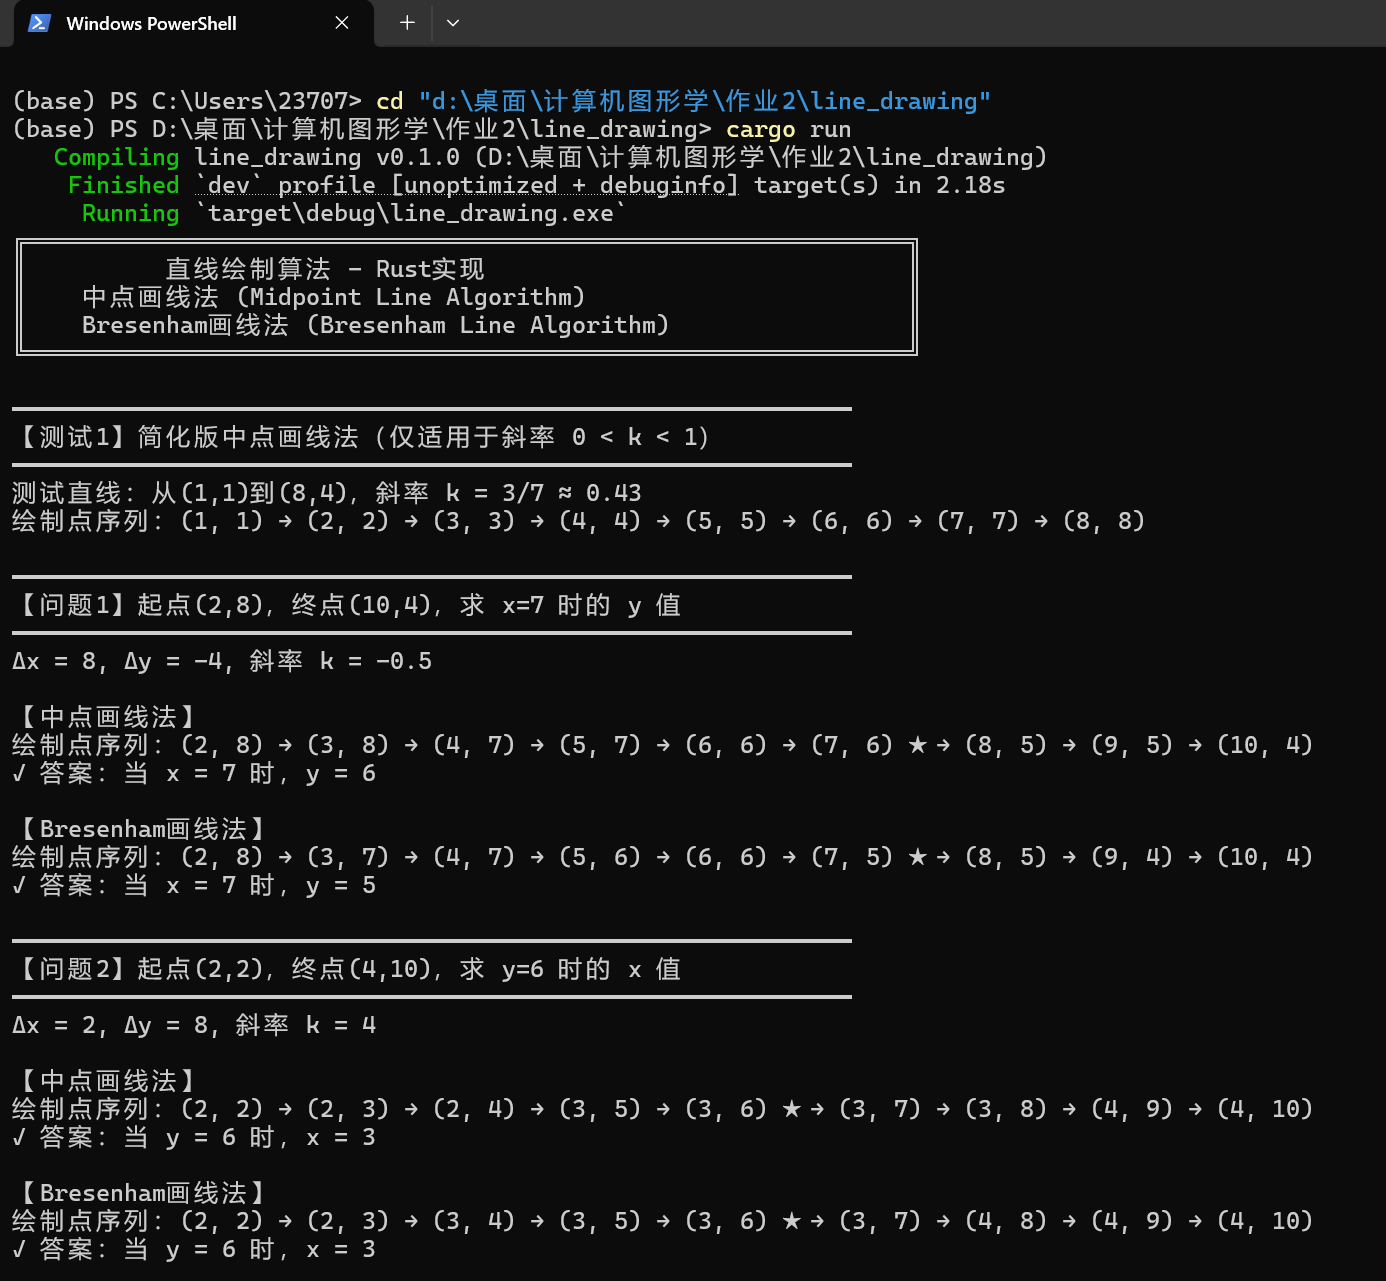
\includegraphics[width=0.95\textwidth]{line_drawing/images/screenshot.png}
\caption{Rust程序运行效果（cargo run输出结果）}
\label{fig:screenshot}
\end{figure}

图\ref{fig:screenshot}展示了Rust程序的运行效果，包含了两个测试问题的完整输出结果。程序清晰地展示了中点画线法和Bresenham画线法对同一直线的不同绘制结果。

\subsubsection{单元测试结果截图}

\begin{figure}[H]
\centering
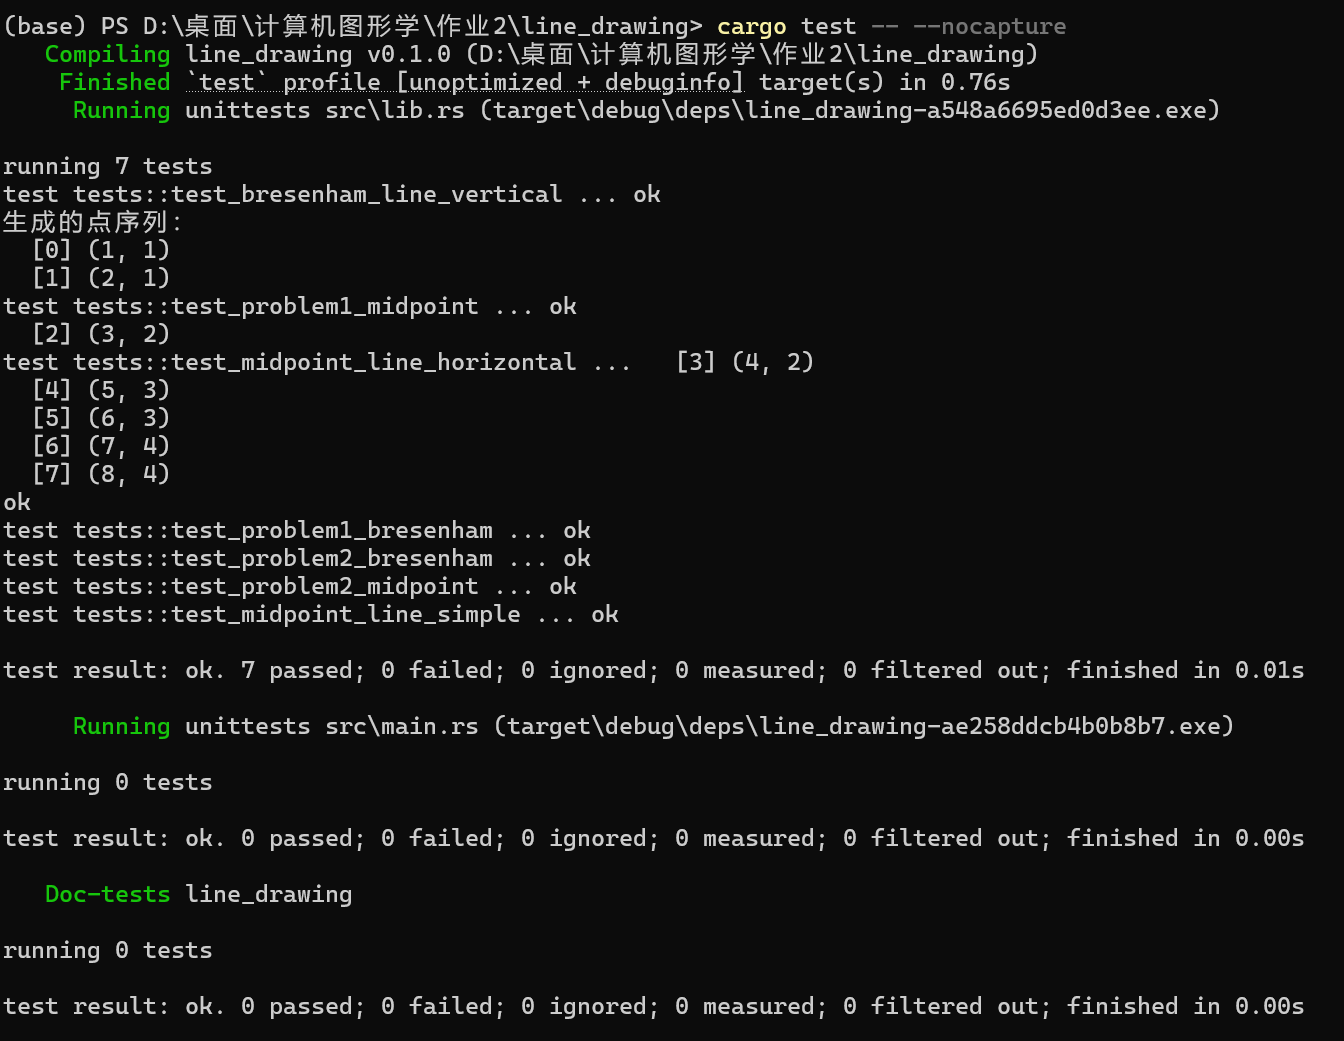
\includegraphics[width=0.95\textwidth]{line_drawing/images/test_result.png}
\caption{单元测试运行结果（cargo test输出）}
\label{fig:test_result}
\end{figure}

图\ref{fig:test_result}展示了所有单元测试的运行结果，验证了算法实现的正确性。测试覆盖了水平线、垂直线、以及两个作业问题的具体情况。

\subsection{算法输出示例}

\begin{tcolorbox}
\textbf{输出：}

\begin{verbatim}
=== 中点画线法：从(2,8)到(10,4) ===
(2, 8) 
(3, 8) 
(4, 7) 
(5, 7) 
(6, 6) 
(7, 6)  <- x=7时，y=6
(8, 5) 
(9, 5) 
(10, 4) 

=== Bresenham画线法：从(2,8)到(10,4) ===
(2, 8) 
(3, 7) 
(4, 7) 
(5, 6) 
(6, 6) 
(7, 5)  <- x=7时，y=5
(8, 5) 
(9, 4) 
(10, 4) 
\end{verbatim}


\end{tcolorbox}

\end{document}
